\documentclass[UTF8,a4paper]{ctexart}%设置a4纸和中文
\ctexset{section/format=\Large\bfseries}%设置标题左对齐
\usepackage{amsmath} % 使用align
\usepackage[margin=1in]{geometry}%设置A4值的边界
\usepackage{graphicx}%插入图片
\usepackage{amsfonts}%使用mathbf
\usepackage{color}
\usepackage{amssymb}
\author{qhy}%作者
\title{机器学习笔记3}%标题
\date{\today}%日期
\pagestyle{empty}%不显示页码
\begin{document}
  \maketitle
  \tableofcontents
  \newpage
  \section{径向基函数网络 Radial Basis Function RBF\color{red}{(样本中心$c_i$这个还需要看一看)}}
    RBF网络,是一种单隐层前馈神经网络,它使用\emph{径向基函数}作为隐层神经元的激活函数,而输出层则是对隐层神经元输出的线性组合。假定输入为$d$维向量$x$,输出为实值,则RBF网络可表示为:
    \begin{equation}
      \varphi(x) = \sum_{i = 1}^q \omega_i \rho(x,c_i)
    \end{equation}
    其中$q$为隐层神经元个数,$c_i$和$w_i$分别是第i个隐层神经元对应的中心和权重,$\rho(x,c_i)$是径向基函数,这是某种沿径向对称的标量函数,通常定义为样本$x$到数据中心$c_i$之间欧氏距离的单调函数。常用的高斯径向基函数形如:
    \begin{equation}
      \rho(x,c_i) = e^{-\beta_i\|x-c_i\|^2}
    \end{equation}
    [Park and Sandberg,1991]证明,具有足够多的隐层神经元的RBF网络能以任意精度逼近任意连续函数。

    通常采用两步过程来训练RBF网络:
    \begin{itemize}
      \item [1.] 确定神经元的中心$c_i$,常用的方式包括随机采样,聚类等
      \item [2.] 利用BP算法等来确定参数$\omega_i$和$\beta_i$
    \end{itemize}

    {\color{blue}
    简单地说,就是使用径向基函数作为隐层的激活函数的单隐层网络,(径向基函数初被用来进行精确的函数内插),每一个径向基函数局部地逼近目标函数的一部分。
    }

  \section{极限学习机 Extream Learning Machine ELM}

      \subsection{简介}

          极限学习机是求解单隐层神经网络的算法。ELM最大的特点,就是对于传统的神经网络,在保证学习精度的前提下比传统的学习算法速度更快。

          该算法在网络参数的确定过程中,除了输出层的权重,其他参数在训练过程中都不进行调整,并且,其初始值也是随机的,而网络外权(即输出权)则是通过最小化均方误差得到的最小二乘解。这样的网络在参数确定的过程中就不需要任何迭代的步骤,从而大大降低了网络参数的调节时间。

      \subsection{原理}
          \subsubsection{人工神经网络应用的理论基础}
              \begin{itemize}
                \item 万能逼近能力定理(Universal Approximation capability) [Leshno 1993, Park and Sandberg 1991, Chen, et al 1995]: 任何连续目标函数可以用前馈神经网络以任意小的误差近似逼近。
                \item 分类能力定理(Classification capability) [Huang, et al 2000]:任何理论上可以分开的目标都可以用人工(前馈)神经网络加以分开。
              \end{itemize}
          \subsubsection{人工神经网络学习的问题核心}
              \begin{itemize}
                \item 这些理论都只是在理论上回答了存在性:给定某种应用存在能提供所需解决能力的对应的人工神经网络结构。
                \item 但这两个定理没有能回答和提供学习的方法(网络结构和算法)。
              \end{itemize}

          \subsubsection{ELM理论}
              面对如此多的神经网络结构,真的需要如此多的不同的对应神经网络算法?
              \begin{itemize}
                \item 不同的前馈网络结构(不仅限于Sigmoid/RBF网络)
                    \begin{itemize}
                      \item sigmoid networks
                      \item RBF networks
                      \item polynomial networks
                      \item complex (domain) networks(复变域网络)
                      \item fourier series(傅立叶变换)
                      \item wavelet networks(小波网络),etc
                    \end{itemize}
                  \item 多层网络(不仅限于多层网络,包括层次性网络)
              \end{itemize}

              生物脑(生物学习系统)中有几十到几百种不同神经元,(其数学模型未知),问题是在生物学习中真的需要调整各种生物神经元?

              ELM学习理论:(机器或生物)学习可以不需要调整隐层节点,给定任何连续目标函数或可分类目标,只要前馈神经的隐层节点是非线性阶段连续的,神经网络无需调整隐层节点就能任意逼近目标连续函数或对分类目标加以分类。

      \subsection{例子}
          对于$m$个的训练样本$(\boldsymbol{x_j},t_j),\boldsymbol{x_j}\in\mathbf{ R }^n,t_j\in\mathbf{ R }$,具有$L$个隐层神经元的单隐层神经网络(图\ref{fig1}),其输出的函数表达式为:
          \begin{equation}
            o_j = \sum_{i = 1}^L \beta_iG(\boldsymbol{ a_i },b_i,\boldsymbol{x_j})
          \end{equation}
          其中,$G(\boldsymbol{a_i},b_i,\boldsymbol{x})$为激活函数,$\beta_i$为输出权,$\boldsymbol{a_i}\in \mathbf{R}^n$为输入权,$b_i$为偏置项
          \begin{figure}[htbp]
            \centering
            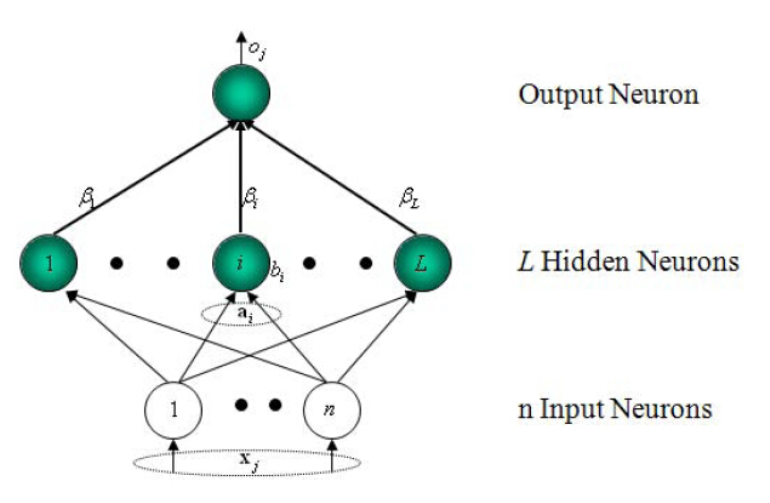
\includegraphics[scale=0.3]{assets/jiqixuexi3_a8b55.png}
            \caption{单隐层前馈神经网络}
            \label{fig1}
          \end{figure}

          单隐层神经网络的输出目标是使得输出的误差最小,
          由万能逼近定理,误差可以达到0,可以表示为:
          \begin{equation}
            E = \sum_{i = 1}^N \| o_j - t_j\| = 0
          \end{equation}
          也就是说,$\exists \beta_i,\boldsymbol{a_i},b_i$使得
          \begin{equation}
            o_j = \sum_{i = 1}^L \beta_iG(\boldsymbol{a_i},b_i,x_j) = t_j
          \end{equation}
          写成矩阵的形式:
          \begin{equation}
            H\beta = T
          \end{equation}
          $H$为隐层节点的输出,$\beta$为输出权重,$T$为目标。
          \begin{equation}
            H =
            \begin{bmatrix}
              G(\boldsymbol{a_1},b_1,x_1) & \cdots & G(\boldsymbol{a_L},b_L,x_1) \\
              \vdots & \ddots & \vdots \\
              G(\boldsymbol{a_1},b_1,x_m) & \cdots & G(\boldsymbol{a_L},b_L,x_m)
            \end{bmatrix}_{m \times L}
            \beta =
            \begin{bmatrix}
              \beta_1\\\vdots\\\beta_L
            \end{bmatrix}_{L\times 1}
            T = \begin{bmatrix}
              t_1^T\\\vdots\\t_m^T
            \end{bmatrix}_{m\times 1}
          \end{equation}
          经推导可以得到 $\hat{\beta} = arg \min_\beta \|H\beta - T\| = H^+T$ {\color{red}这个结论怎么得到的?还需要去推导}

  \section{降维与度量学习}
      \subsection{k近邻学习 k-Nearest Neighbor kNN}
          \subsubsection{简介}
              k近邻(\emph{k-Nearest Neighbor} , 简称\emph{kNN})学习是一种常用的监督学习方法,其工作机制非常简单:给定测试样本,基于某种距离度量找出训练集中与其最靠近的k个训练样本,然后基于这k个"邻居"的信息进行预测。

              在分类任务中,可使用投票法,即选择这k个样本中出现最多的类别标记作为预测结果。

              在回归任务中,可使用平均法,即将这k个样本的实值输出标记的平均值作为预测结果。

              还可以基于距离远近进行加权平均或加权投票,距离越近的样本权重越大。

          \subsubsection{懒惰学习与急切学习}
              与其他的学习方法相比,k近邻学习有一个明显的不同之处,它没有显示的训练过程。这称为 \emph{懒惰学习 lazy learning}即在训练阶段,它仅仅是把样本保存起来,训练时间开销为0,待收到测试样本之后再进行处理。

              相应的,那些在训练阶段就对样本进行学习处理的方法,称为\emph{急切学习 eager learning}
          \subsubsection{学习效果分析}
              给定测试样本$\mathbf{x}$,若其最近邻样本为$\mathbf{z}$,则最近邻分类器出错的概率就是$\mathbf{x}$与$\mathbf{z}$类别标记不同的概率,即
              \begin{equation}
                  P(err) = 1 - \sum_{c \in y}P(c|\mathbf{x})P(c|\mathbf{z})
                  \label{perrofknn}
              \end{equation}
              {\color{red}{为啥是用后验概率呀?}}

              假设样本独立同分布,且对任意$\mathbf{x}$和任意小的$\delta$,在$\mathbf{x}$附近$\delta$距离范围内总能找到一个训练样本;换言之,对任意测试样本,总能在任意近的范围内找到式\eqref{perrofknn}中的训练样本$\mathbf{z}$。

              令$c^* = arg \max_{c\in y}P(c|x)$表示贝叶斯最优分类器的结果,有

              \begin{align}
                P(err) &= 1 - \sum_{c \in y}P(c|\mathbf{x})P(c|\mathbf{z}) \\
                       &\simeq 1 - \sum_{c \in y}P^2(c|\mathbf{x})\\
                       &\leqslant 1 - P^2(c^*|\mathbf{x})\\
                       &= (1 + P(c^*|\mathbf{x}))(1 - P(c^*|\mathbf{x}))\\
                       &\leqslant 2\times (1 - P(c^*|\mathbf{x}))
              \end{align}

              {\color{red}{贝叶斯最优分类器需要去看}}

              也就是说,最近邻分类器它的繁华错误不超过贝叶斯最优分类器的错误率的两倍。

          \subsubsection{维数灾难 curse of dimensionality}
              上一节的讨论是基于一个重要的假设:任意测试样本$\mathbf{x}$附近任意小的$\delta$距离范围内总能找到一个训练样本。
              也就是说,训练样本的采样密度要足够大,或称为\textbf{密采样}

              然而,这个假设在现实任务中通常很难满足,现实应用中的属性维数经常成千上万,要满足密采样条件所需的样本数目是无法达到的天文数字。

              此外,许多学习算法都涉及距离计算,而高维度空间会给距离计算带来很大的麻烦。

              事实上,在高维情况下,出现的数据样本稀疏,距离计算困难等问题是所有机器学习方法共同面临的严重障碍,被称为\textbf{维数灾难 curse of dimensionality}

              {\color{blue}
                  另一方面,在高维的情况,为达到好的训练效果,那么就需要更多的样本以适应更多的属性;
              }

              解决维度灾难的一个重要途径是\textbf{降维 dimension reduction},亦称为\textbf{维数简约},即通过某种数学变换,将原始高维属性空间转换为一个低维子空间。

      \subsection{多维缩放 Multiple Dimensional Scaling MDS}
          \subsubsection{低维嵌入}
              为什么能进行降维?
              在很多时候,人们观测或者收集到的数据样本虽是高维的,但与学习任务密切相关的也许仅是某个低维分布,即高维空间中的一个\textbf{低维嵌入 embedding}。 图\ref{figembedding}是一个直观的例子。

              \begin{figure}[htbp]
                \centering
                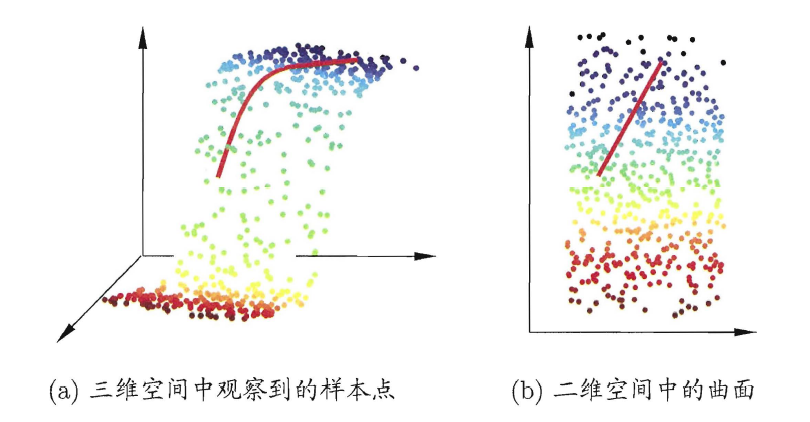
\includegraphics[scale=0.5]{assets/jiqixuexi3_9102e.png}
                \caption{低维嵌入示意图}
                \label{figembedding}
              \end{figure}

              {\color{blue}{ 根据上面的说法,最简单的降维思路,就是人工把不需要的属性去掉,只取认为有用的属性进行学习 }}

              {\color{red}{ 但是,大部分情况我们并不知道哪些属性,后面的算法中,根据什么东西来选择哪些属性,这样选择的意义在哪里,为什么这么选择能得到需要的低维样本,需要进一步的思考 }}

          \subsubsection{MDS 推导过程}
              MDS是一种经典的降维方法,它的目的是,尽可能保证原始空间中样本的距离在低维空间中得以保持。{\color{blue}{也就是说,样本"投影"到低维空间之后,样本之间的距离尽可能地保持一样。}}

              下面是推导过程:
              假设$m$个样本在原始空间的距离矩阵为$D\in \mathbb{R}^{m\times m}$,第$i$行第$j$列的元素$dist_{ij}$为样本$\mathbf{x_i}$到$\mathbf{x_j}$的距离。
              我们的目标是获得样本在$d'$维空间的表示$Z\in \mathbb{R}^{d'\times m} , d' \leqslant d$且任意两个样本在$d'$维空间中的欧式距离等于原始空间中的距离,即$\|z_i - z_j\| = dist_{ij}$

              {\color{red}
                是否一定存在这样的$d'$维空间?比如四面体怎么嵌入到一个二维平面?貌似无法保持边与边的关系,后面实验看看是什么情况?
              }

              令$\mathbf{B = Z^TZ} \in \mathbb{R}^{m\times m}$,其中$\mathbf{B}$为降维后样本的内积矩阵,$b_{ij} = \mathbf{z_i^Tz_j}$,有

              \begin{align}
                dist_{ij}^2 &= \|\mathbf{z_i}\|^2 + \|\mathbf{z_j}\|^2 - 2\mathbf{z_i}^T\mathbf{z_j}  \\
                          &= b_{ii} + b_{jj} - 2b_{ij}
                \label{distijbiibjj2bij}
              \end{align}


              为方便讨论,令降维后的样本被中心化, 即$\sum_{i = 1}^m \mathbf{z_i} = 0$,显然矩阵B的行和列之后也均为零。即:
              \begin{align}
                \sum_{i = 1}^m b_{ij} = \sum_{i = 1}^m \mathbf{z_i}^T\mathbf{z_j} = \left ( \sum_{i = 1}^m \mathbf{z_i}^T \right)\mathbf{z_j} = 0\\
                \sum_{j = 1}^m b_{ij} = \sum_{j = 1}^m \mathbf{z_i^Tz_j} = \mathbf{z_i}\left ( \sum_{i = 1}^m \mathbf{z_j^T} \right) = 0
              \end{align}

              易知:
              \begin{align}
                  \sum_{i = 1}^m dist_{ij}^2 = tr(\mathbf{B}) + mb_{jj} \label{distijBmbjj}\\
                  \sum_{j = 1}^m dist_{ij}^2 = tr(\mathbf{B}) + mb_{ii}\label{distijBmbii}\\
                  \sum_{i = 1}^m  \sum_{j = 1}^m dist_{ij}^2 = 2m tr(\mathbf{B})
                  \label{distij2mb}
              \end{align}
              其中,$tr(B) = \sum_{i = 1}^m b_{ii} = \sum_{i = 1}^m \| \mathbf{z_i} \|^2$

              由式\eqref{distijbiibjj2bij} \eqref{distijBmbjj} \eqref{distijBmbii} \eqref{distij2mb}得:
              \begin{align}
                b_{ij} &= -\frac{1}{2} \left ( dist^2_{ij} - b_{ii} - b_{jj} \right ) \\
                &= -\frac{1}{2} \left ( dist^2_{ij} - \frac{\sum_{k = 1}^m dist_{ik}^2  - tr(B)}{m} - \frac{\sum_{k = 1}^m dist_{kj}^2  - tr(B)}{m} \right ) \\
                &= -\frac{1}{2} \left ( dist^2_{ij} - \frac{\sum_{k = 1}^m dist_{ik}^2  }{m} - \frac{\sum_{k = 1}^m dist_{kj}^2}{m} + \frac{2tr(B)}{m} \right )\\
                &= -\frac{1}{2} \left ( dist^2_{ij} - dist^2_{i\cdot} - dist^2_{\cdot j} +  dist_{\cdot \cdot}^2 \right ) \label{bijdijdi*d*jd**}
              \end{align}

              其中
              \begin{align}
                  dist^2_{i\cdot} =  \frac{1}{m}\sum_{k = 1}^m dist_{ik}^2 \label{disti*}\\
                  dist^2_{\cdot j} = \frac{1}{m}\sum_{k = 1}^m dist_{kj}^2\label{dist*j}
              \end{align}
              \begin{equation}
                \label{dist**}
              \begin{split}
                  dist^2_{\cdot \cdot} &=\frac{1}{m^2} \sum_{s = 1}^m \sum_{t = 1}^m dist_{st}^2 \\
                  &= \frac{1}{m^2} \sum_{s = 1}^m \sum_{t = 1}^m (b_{ss} + b_{tt} - 2b_{st})\\
                  &= \frac{1}{m^2} \sum_{s = 1}^m \sum_{t = 1}^m (b_{ss} + b_{tt})\\
                  &= \frac{1}{m^2} \left (   \sum_{t = 1}^m  \sum_{s = 1}^m b_{ss} + \sum_{s = 1}^m \sum_{t = 1}^m b_{tt} \right )\\
                  &= \frac{1}{m^2} \sum_{t = 1}^m 2mb_{tt}\\
                  &= \frac{2}{m} \sum_{i = 1}^m \| \mathbf{z_i} \|^2 \\
                  &= \frac{2}{m} tr(\mathbf{B})
              \end{split}
              \end{equation}

              由此,$\mathbf{B}$矩阵就能通过样本的距离矩阵确定
              对$\mathbf{B}$矩阵进行特征值分解:$\mathbf{B} = V\Lambda V^T$
              其中$\Lambda = diag(\lambda_1,\lambda_2,\cdots,\lambda_d)$为特征值构成的对角矩阵,$\lambda_1\geqslant \lambda_2\geqslant\cdots\geqslant\lambda_d$
              $\Lambda$为特征向量矩阵。

              $\mathbf{\mathbf{B}} = \mathbf{Z^TZ}$

              假定其中有$d^*$个非零特征值,它们构成对角矩阵$\Lambda_* = diag(\lambda_1,\lambda_2,\cdots,\lambda_{d^*})$,令$V_*$表示相应的特征向量矩阵,则Z可以表示为
              \[ \mathbf{Z} =\Lambda_*^{1/2}V_*^T \in \mathbb{R}^{d^* \times m}  \]

              {
              \color{red} 特征值为0的情况,是不是说明样本中,有某两个维度表示的是同一个属性?
              }

              在现实应用中,为了有效降维,往往仅需降维后距离与原始空间距离尽可能相近,而不必严格相等。

              此时,可以取$d' << d$个最大特征值构成对角矩阵,$\tilde{\Lambda } = diag(\lambda_1,\lambda_2,\cdots,\lambda_{d'} )$,令$\tilde{V}$表示相应的特征向量矩阵,则Z可以表示为
                \[ \mathbf{Z} =\tilde{\Lambda}^{1/2}\tilde{V}^T \in \mathbb{R}^{d' \times m}  \]

                {\color{red}
                    结果看起来像是直接开方,具体运算细节还需要学习。
                }
                {\color{red}
                  特征值越大,是不是说明这个特征向量对矩阵的所占的比重越大?需要查查特征值和特征向量的意义加深理解。
                }

            \subsubsection{MDS 算法}
            \begin{tabular}{l}
              \hline
              \textbf{输入:}距离矩阵$\mathbf{D} \in \mathbb{R}^{m \times m}$,其元素$dist_{ij}$为样本$\mathbf{x_i}$到$\mathbf{x_j}$的距离:
              {\color{red}等等,不需要对样本先进行中心化处理吗?}\\
            \textbf{过程:}\\
              1: 根据式\eqref{disti*},\eqref{dist*j},\eqref{dist**} 计算$    dist^2_{i \cdot},  dist^2_{\cdot j},dist^2_{\cdot \cdot}$\\
              2: 根据式\eqref{bijdijdi*d*jd**}计算矩阵$\mathbf{B}$\\
              3: 对矩阵$\mathbf{B}$做特征值分解\\
              4: 取$\tilde{\Lambda}$为$d'$个最大特征值所构成的对角矩阵,$\tilde{V}$为相应的特征向量矩阵\\
              \textbf{输出:}矩阵$\tilde{\Lambda}^{1/2}\tilde{V}^T \in \mathbb{R}^{d' \times m}$,每一列是一个样本的低维坐标。{\color{red} 西瓜书是$\tilde{\tilde{V}^\Lambda}^{1/2} \in \mathbb{R}^{m \times d'}$,把两个量交换了位置,不知道这么写有什么深意。}\\
              \hline
            \end{tabular}
      \subsection{主成分分析 Principal Component Analysis PAC}
          \subsubsection{线性降维方法}
              一般来说,欲获得低维子空间,最简单的是对原始空间进行线性变换。

              给定$d$维空间中的样本$X = {x_1,x_1,\cdots ,x_m} \in \mathbb{R}^{d\times m }$,变换之后得到$d' \leqslant d$维的空间中的样本:
              \begin{equation}
                \mathbf{Z = W^TX}
              \end{equation}
              其中$\mathbf{W}\in \mathbb{R}^{d\times d'}$是变换矩阵,$\mathbf{Z}\in \mathbb{R}^{d' \times m}$是样本在新空间中的表达。

              {\color{blue}
                  这里Z的每一维度的坐标,都是原始空间上的所有坐标的一个线性组合,这个值可以看成是新低维空间中,当前前以变换矩阵中某一列为基的值。

                  \textbf{矩阵乘法的物理意义:}将右边矩阵中的每一列列向量变换到左边矩阵中每一行行向量为基所表示的空间中去

                  从另一个角度来理解的话,降维是对样本在原始空间上进行一定的转换,再根据某个评价标准(比如特征值的大小),取转换后的样本的一部分维度作为低维空间的组成。
              }

              基于线性变换来进行降维的方法,称为\textbf{线性降维方法}
          \subsubsection{PAC 简介}
              PAC是有种线性降维方法,它要求降维后的样本具有最大的可分性。

          \subsubsection{基于最近重构性的推导}

          \subsubsection{基于最大可分性的推导}

          \subsubsection{PAC 算法}

      \subsection{核主成分分析 Kernelized PAC KPAC}
          \subsubsection{KPCA 简介}
              KPCA的想法是,先把数据升维,再进行降维操作。

              {\color{blue}
              在降维的时候,我们希望在保持原有特性的情况下,把样本映射到低维空间来达到减小时间开销的目的,但是如果样本的特性不明显,或者是降维之后特性消失了,那么降维之后的学习效果就不会很好。

              基于高维空间往往更线性可分的想法,可以考虑把样本先升维到高维空间,使得样本的特性更加明显,再进行降维。

              核主成分分析就是把样本映射到了高维空间,再进行降维操作。
              }

          \subsubsection{KPCA 推导}


    \section{核函数}
        核函数:高维空间和低维空间的一个桥梁,从效果上看,就是把低维空间的样本映射到了高维空间,高维空间的计算,则是通过核函数来进行,避免了维数灾难的问题。
\end{document}
